\section{Auswertung}
\label{sec:auswertung}

Die aufgenommenen Messdaten werden mithilfe der Python-Pakte Matplotlib \cite{matplotlib} und NumPy \cite{numpy}
ausgewertet. Fehlerrechnung in erster Ordnung wird mittels \cite{uncertainties} automatisiert.

\subsection{Magnetfeld}

Die aufgenommen Messwerte der magnetische Flussdichte werden in der Tabelle \ref{tab:feld} dargestellt.
Es wurde die Flussdichte $B$ an der jeweiligen Position $z$ notiert.
Die Reihenfolge in der die Werte dargestellt sind entspricht auch der Reihenfolge in der die Messwerte aufgenommen wurden.
Dabei wurde die Mitte in dem Luftspalt per Auge abgeschätzt.

\begin{table}[H]
	\centering
	\caption{Messwerte der magnetischen Flussdichte um den Luftspalt.}
	\input{build/table_field.tex}
	\label{tab:feld}
\end{table}

Zur Bestimmung der maximalen Flussdichte werden die in der Tabelle \ref{tab:feld} angegebenen Werte in dem
Plot \ref{fig:feld} aufgetragen.

\begin{figure}[H]
    \centering
    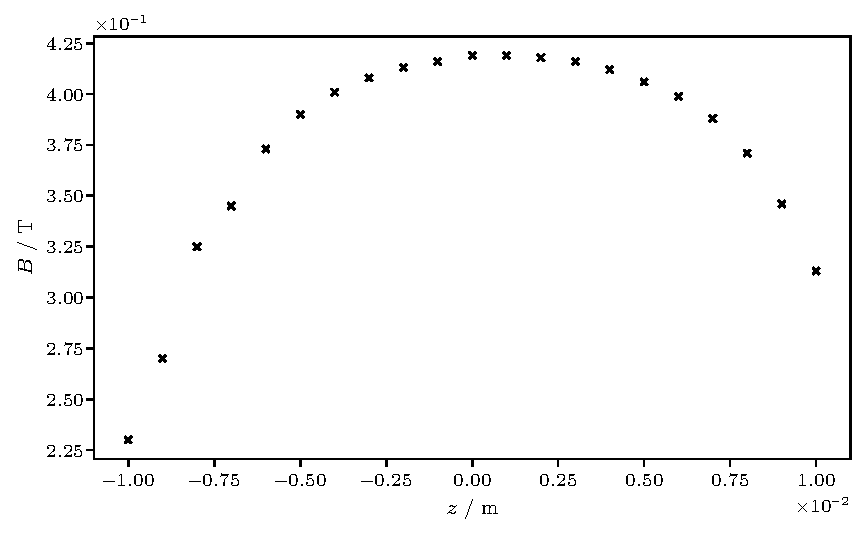
\includegraphics{build/field.pdf}
    \caption{Messung zum Verlauf des Magnetfeldes um den Luftspalt.}
    \label{fig:feld}
\end{figure}

Der Maximalwert der magnetischen Flussdichte lässt anhand des Plots \ref{fig:feld} ablesen und beträgt
\qty{419}{\milli\tesla}.

\subsection{Faraday-Rotation}

Es wurden drei unterschiedliche Proben verwendet. Die jeweiligen Messwerte der Proben für die unterschiedlichen Interferenzfilter werden
in Tabelle \ref{tab:proben} dargestellt.

\begin{table}[H]
	\centering
	\caption{Messwerte der Rotationswinkel für beide Feldrichtungen.}
	\input{build/table_samples.tex}
	\label{tab:proben}
\end{table}

\subsubsection{Dotierte Proben}
\label{sec:Dotierte}

Es werden zunächst zwei verschiende Dotierungsstärken des Galliumsarsenids ausgewertet. Die mit n-GaAs (1) bezeichnete
Probe hat die Eigentschaften $N = \qty{1.2e18}{\per\centi\meter\cubed}$ und $L = \qty{1.36}{\milli\meter}$. Die mit n-GaAs (2)
bezeichnete Probe hat die Eigenschaften $N = \qty{2.8e18}{\per\centi\meter\cubed}$ und $L = \qty{1.296}{\milli\meter}$.

Für n-GaAs (1) wurde die Differenz der Messwerte auf eine Feldstärke von $B$ an Stelle von $2 \cdot B$ normiert.
Anschließend wurden diese normierten Werte gegenüber der Wellenlänge der Interferenzfilter zum Quadrat im
Plot \ref{fig:dotiert-1} aufgetragen.

\begin{figure}[H]
    \centering
    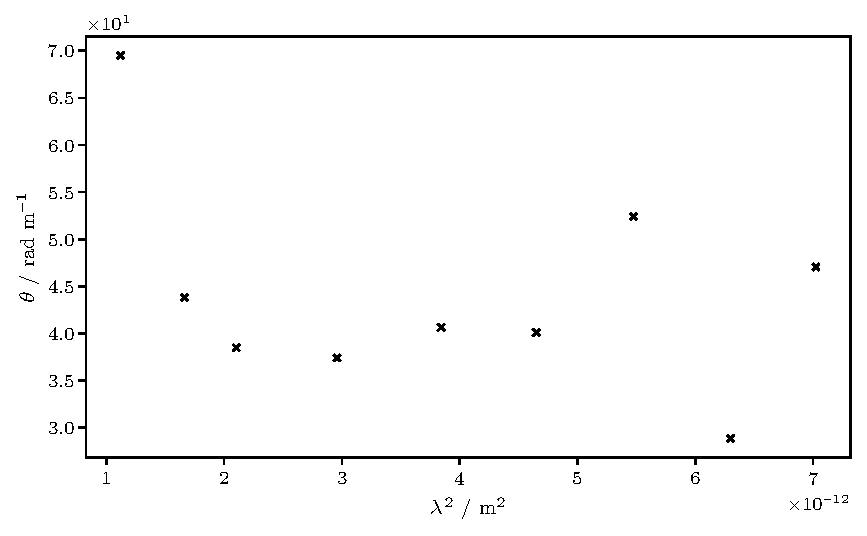
\includegraphics{build/doped-1.pdf}
    \caption{Messung zum normierten Drehwinkel für n-GaAs (1).}
    \label{fig:dotiert-1}
\end{figure}

Für n-GaAs (2) wurde die Differenz der Messwerte auf gleicher Weise normiert.
Dies wird äquivalent wie in Abbildung \ref{fig:dotiert-1} im Plot \ref{fig:dotiert-2} aufgetragen.

\begin{figure}[H]
    \centering
    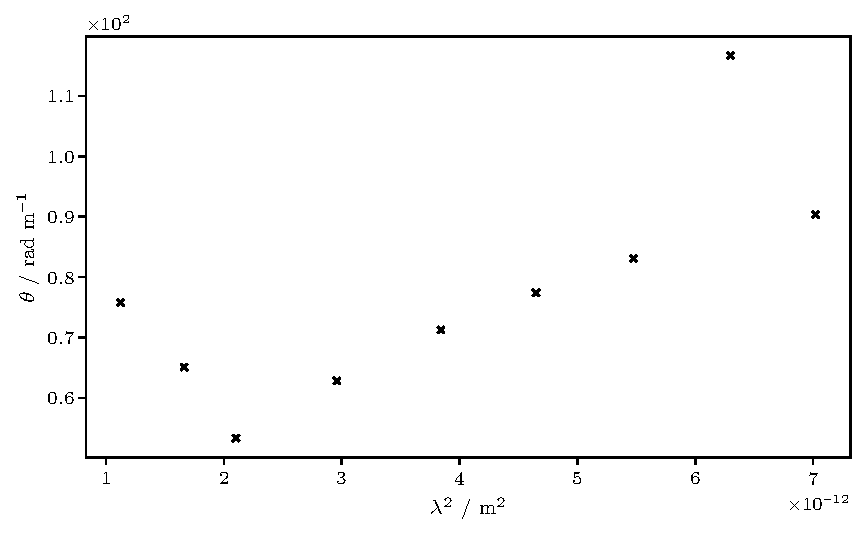
\includegraphics{build/doped-2.pdf}
    \caption{Messung zum normierten Drehwinkel für n-GaAs (2).}
    \label{fig:dotiert-2}
\end{figure}

\subsubsection{Reine Probe}

Die hochreine GaAs Probe hat eine Dicke von $L = \qty{5.11}{\milli\meter}$.
Für die Messwerte der reinen GaAs Probe wurde wie in Abschnitt \ref{sec:Dotierte} verfahren.
Anschließend wurden die Winkel-Werte gegenüber der Wellenlänge der Interferenzfilter zum Quadrat in Plot \ref{fig:rein}
aufgetragen.

\begin{figure}[H] 
    \centering
    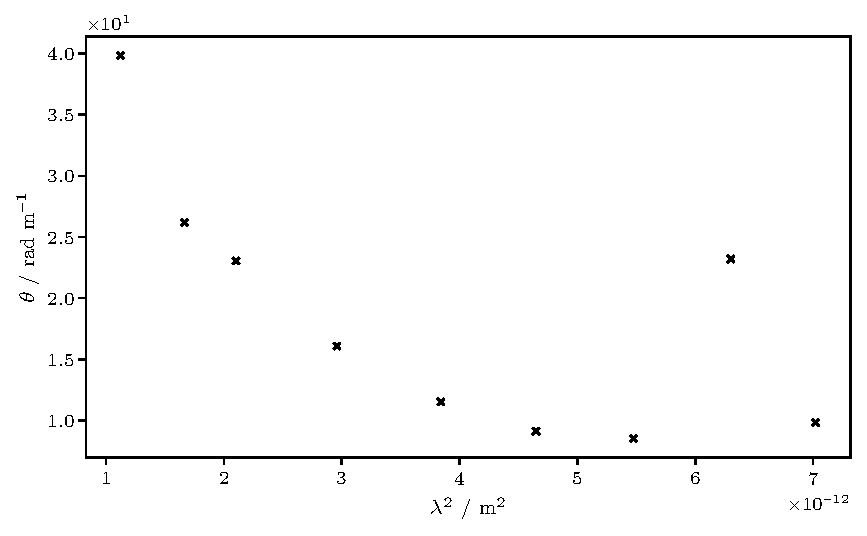
\includegraphics{build/pure.pdf}
    \caption{Messung zum normierten Drehwinkel für GaAs.}
    \label{fig:rein}
\end{figure}

\subsection{Effektive Masse}

Anhand \eqref{eqn:ausgleichsrechnung} lässt sich eine Ausgleichsgerade der Form
\begin{align*}
    \pfrac{\theta}{L} = a \lambda^2 + b
\end{align*}
an die Messdaten legen. Der Parameter $b$ erlaubt dabei für eine Veschiebung der Ergebnisse und kompensiert somit derartige
Ungenauigkeiten aus dem Versuchsaufbau. Der Koeffizient $a$ lässt sich nach $m^{*}$ auflösen, sodass
\begin{align}
    m^* = \sqrt{\pfrac{Ne_0^3B}{8\pi^2 \varepsilon_0 c^3 n a}} \label{eqn:final}
\end{align}
die effektive Masse beschreibt. Dazu werden die Naturkonstanten $c = \input{build/c.tex}$,
$e_0 = \input{build/e-0.tex}$, $m_0 = \input{build/m-0.tex}$ sowie die Materialeigenschaft
$n = \num{3.397}$ \cite{brechungsindex} benötigt.

Für die Winkeldifferenz aus GaAs und n-GaAs (1) folgen
\begin{align*}
    a = \input{build/a-1.tex} && b = \input{build/b-1.tex}
\end{align*}
aus der Ausgleichsrechnung. Analog lassen sich
\begin{align*}
    a = \input{build/a-2.tex} && b = \input{build/b-2.tex}
\end{align*}
für GaAs und n-GaAs (2) bestimmen. Beim Fitting werden einige Datenpunkte ignoriert, im folgenden Abschnitt gehen wir näher
darauf ein.

\begin{figure}[H]
    \centering
    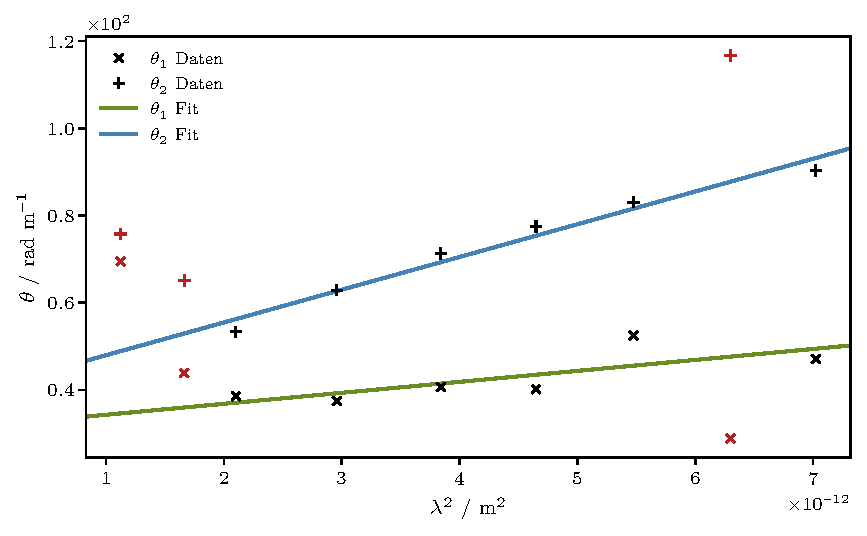
\includegraphics{build/mass.pdf}
    \caption{Messergebnisse und Ausgleichgeraden zum Drehwinkel aus Wirkung der Leitungselektronen.
             Ausgelassene Datenpunkte sind hervorgehoben.}
    \label{fig:masse}
\end{figure}
